
\chapter{Proposal}
\section{Problem statement}
An escape room is a type of a game, where one has to solve a set of puzzles to escape from a locked room.
These puzzles are connected together to form a narrative, and their correct interaction is necessary for the proper telling of the plot. The players interact with the puzzles in a non-strictly sequential way, so that the whole game can be modeled as an event based system. If these puzzles don't work as intended, the customer will be dissatisfied, so it's crucial to ensure that no dead-locks occur due to their unpredictable interactions with the system. The expected result is an event based model of player interaction, which would allow for the staff to monitor player progress, and potentially for easier extension of the game.
\section{Work plan}
An expected time frame of development is shown below, milestones are marked in bold:
\begin{enumerate}
        \item Description of physical elements of the system, and their interactions - Tomasz L., Krzysztof K.- 13.11
        \item \textbf{Modeling the system using a Petri net - Jacek G., Tomasz M. - 27.11}
        \item Using the petri model to find issues in the system - Tomasz L., Michał K. - 4.12
        \item \textbf{Checking the model against a simulated escape room based on a real one - Whole Team - 8.01} 
            \begin{itemize}
                \item Specific
                \item Tasks
                \item to
                \item be
                \item discussed
            \end{itemize}
        \item Delivery of results - Michał K. - 22.01
\end{enumerate}



\begin{figure}[h!]
    \centering
    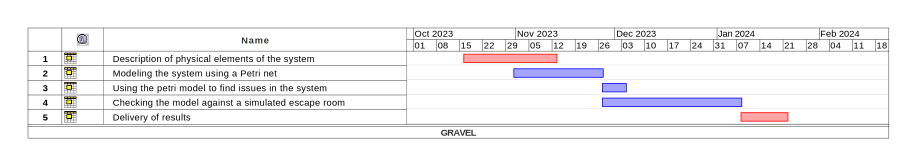
\includegraphics[width=1.0\textwidth]{GRAVEL.pdf}
    \caption{Gantt chart of the work plan}
\end{figure}

\section{Delivery}
The first milestone will cover the following:
\begin{itemize}
    \item A description of an example escape room, its story, puzzles - as well as elements comprising them - will be provided in the report. The example will be based on one which was already implemented in practice.
    \item A Petri net model of player-system interaction will be created and described in the report.
\end{itemize}
The second milestone will cover:
\begin{itemize}
    \item A report describing the use of the Petri model to find possible issues - Deadlocks, loops, etc. - as well as possible fixes for them. 
    \item Source code of the simulation, its results, and report of its design.
\end{itemize}

Finally, a report discussing the project as a whole will be provided at its end. The project will be disclosed in its entirety, however due to the use of real systems for event-based description, it may not be published or used in any way other than what's necessary for the course.

\section{Team}
The management structure of the team is as follows:\\

\begin{center}
    \begin{tikzpicture}[block/.style = {draw, fill=white, rectangle, minimum height=3em, minimum width=3em},
    adv/.style= {draw, fill=green!30, circle, node distance=5mm},
    part/.style= {draw, fill=blue!30, circle, node distance=1mm},
    words/.style = {draw, fill = white, rectangle,node distance=5mm},
    tmp/.style = {coordinate,node distance=10mm},
    pinstyle/.style = {pin edge={to-,thin,black}},
    auto,
    node distance = 2cm,
    >=latex'
    ]
    
    

    \node [tmp, name=center](center){};
    \node [words,right=of center](output)
            {
                Leader - Krzysztof Kowaczek
            };
    \draw [->] (center) --  (output);
    
        \node [tmp, above=of center] (advslave)
            {
                
            };
        \node [words, name=wordsslave, left=of advslave] (wordsslave)
            {
                Jacek Grzegorzewski
            };
        \draw [--] (advslave) -|  (center);
        \draw [--] (wordsslave) -|  (advslave);
     
        \node [tmp, above=of advslave] (advslave1)
            {
                
            };
        \node [words, name=wordsslave1, left=of advslave1] (wordsslave1)
            {
                Tomasz Marut
            };
        \draw [--] (advslave1) -|  (center);
        \draw [--] (wordsslave1) -|  (advslave1);
    
        \node [tmp, below=of center] (advslave2)
            {
                
            };
        \node [words, name=wordsslave2, left=of advslave2] (wordsslave2)
            {
                Michał Kos
            };
        \draw [--] (advslave2) -|  (center);
        \draw [--] (wordsslave2) -|  (advslave2);
    
        \node [tmp, below=of advslave2] (advslave3)
            {
                
            };
        \node [words, name=wordsslave3, left=of advslave3] (wordsslave3)
            {
                Tomasz Lubelski
            };
        \draw [--] (advslave3) -|  (center);
        \draw [--] (wordsslave3) -|  (advslave3);



    \end{tikzpicture}
\end{center}
\\
Progress will be monitored by Tomasz Marut, who's also obligated himself to solving inter-member conflicts by physical punishment. Regular meetings will be held at the round table (SKS), where printed documents will be exchanged - we do not plan on keeping any digital copies, as we fear the temporary nature of the digital world. The team coordinator has the power to bear responsibility for other member's shortcomings, as well as the privilege of being on the right side of the org chart. The team coordinator will project his mind astrally to each team member at full moon - this may cause issues if mercury is in retrograde, as Leo's don't work well with mercury. Intellectual property is equally shared among all team members, who will have to decide by majority if it should be be granted to a third party.

\subsection{Responsibility for failure}
All responsibility for failure of the above described project
falls upon team members not present at the time of writing this document
- 30.10.23	16:20:35-CET - 
who, by remaining silent when asked, agreed to this responsibility.
The following team members bare the burden of failure:
\begin{itemize}
    \item Michał Kos
    \item Tomasz Lubelski
\end{itemize}



